\chapter{Лабораторная работа №1\\
Измерение мощности СВЧ}

\section{Цель работы}

\begin{enumerate}
    \item На примере измерений мощности СВЧ усвоить смысл, содержание, определение основных понятий радиоизмерений на высоких и сверхвысоких частотах:
        \begin{itemize}
            \item измеряемая физическая величина (ФВ);
            \item принцип измерений;
            \item метод измерений, уравнение измерений;
            \item измерительная задача;
            \item структура измерительного прибора;
            \item составные части радиоизмерительного прибора --- мера ФВ, преобразователь, устойствро сравнения, устройство визуализации --- отображение результата;
            \item погрешность измерения;
            \item физические явления, влияющие на результат и погрешность измерения;
            \item погрешность измерительного прибора;
            \item условия измерений.
        \end{itemize}

    \item Изучить и усвоить основные теоретические сведения об измерениях мощности СВЧ.

    \item Научиться самостоятельно готовиться к решению поставленной инженерной измерительной задачи.

    \item Освоить навыки самостоятельной работы с измерителем мощности и генератором излучения СВЧ.
\end{enumerate}

% \section{Теоретические сведения}

\section{Практическая часть}

\subsection{Измерительная задача №1}

Согласно методике определим зависимость выходной мощности генератора Г4-82 от частоты в диапазоне частот от $5.6~\text{ГГц}$ до $7.5~\text{ГГц}$.
Заполним на основании этих данных таблицу~\ref{tab:frequency-to-power}.

\begin{table}[H]
    \centering
    \caption{Зависимость выходной мощности $P$ от частоты $f$}%
    \label{tab:frequency-to-power}
    \resizebox{\textwidth}{!}{%
        \begin{tabular}{@{}lcccccccccccccccccccc@{}}
            \toprule
            $f\text{, ГГц}$            & 5.6   & 5.7   & 5.8   & 5.9   & 6.0   & 6.1   & 6.2   & 6.3   & 6.4   & 6.5   & 6.6   & 6.7   & 6.8   & 6.9   & 7.0   & 7.1   & 7.2   & 7.3   & 7.4   & 7.5   \\ \midrule
            \rowcolor[HTML]{C0C0C0}
            $P_1\text{, мВт}$          & 1.020 & 1.161 & 1.782 & 1.726 & 1.502 & 1.762 & 1.675 & 1.842 & 1.710 & 1.439 & 1.360 & 1.375 & 1.370 & 0.974 & 1.053 & 0.591 & 0.002 & 0.002 & 0.002 & 0.002 \\
            $P_2\text{, мВт}$          & 1.023 & 1.162 & 1.783 & 1.721 & 1.506 & 1.765 & 1.684 & 1.856 & 1.710 & 1.448 & 1.369 & 1.382 & 1.377 & 0.934 & 1.058 & 0.596 & 0.002 & 0.002 & 0.002 & 0.002 \\
            \rowcolor[HTML]{C0C0C0}
            $P_3\text{, мВт}$          & 1.016 & 1.154 & 1.776 & 1.721 & 1.507 & 1.758 & 1.687 & 1.855 & 1.706 & 1.444 & 1.357 & 1.372 & 1.382 & 0.950 & 1.070 & 0.592 & 0.002 & 0.002 & 0.002 & 0.002 \\
            $\overline{P}\text{, мВт}$ & 1.020 & 1.159 & 1.780 & 1.723 & 1.505 & 1.762 & 1.682 & 1.851 & 1.709 & 1.444 & 1.362 & 1.376 & 1.376 & 0.953 & 1.060 & 0.593 & 0.002 & 0.002 & 0.002 & 0.002 \\
            \bottomrule
        \end{tabular}%
    }
\end{table}

Пользуясь вычисленным средним значением, построим зависимость выходной мощности $P$ от частоты $f$ (Рис.~\ref{fig:frequency-to-power}).
\begin{figure}[H]
    \centering
    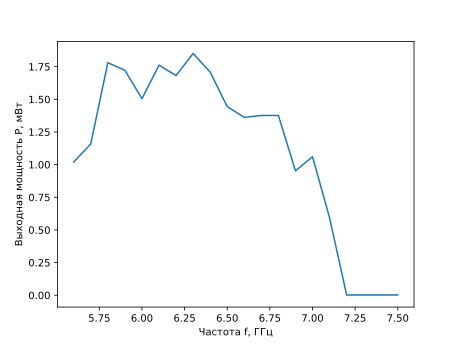
\includegraphics[width=0.8\textwidth]{frequency-to-power.pdf}
    \caption{Зависимость выходной мощности $P$ от частоты $f$}%
    \label{fig:frequency-to-power}
\end{figure}

По графику можно сделать вывод, что наилучшее согласование обеспечивается в диапазоне частот $5.8-6.3~\text{ГГц}$.

\subsection{Измерительная задача №2}

Определим случайную погрешность измерения мощности генератора при помощи ваттметра поглощаемой мощности на частоте $f = 6~\text{ГГц}$ при пределах измерений $P_1 = 0.5~\text{мВт}$ и $P_2 = 5.0~\text{мВт}$.
На основе полученных данных рассчитаем среднее значение мощности $P_\text{ср}$, среднее квадратическое отклонение результата единичного измерения и среднее квадратическое отклонение значения $P_\text{ср}$.
Данные занесём в таблицу~\ref{tab:power-to-power-limit}.

\begin{table}[H]
    \centering
    \caption{Случайная погрешность измерений мощности генератора при помощи ваттметра поглощаемой мощности}%
    \label{tab:power-to-power-limit}
    \resizebox{\textwidth}{!}{%
        \begin{tabular}{@{}ccccccccccccccc@{}}
            \toprule
            Предел измерений, мВт & \multicolumn{10}{c}{Измеренная мощность, мВт}                                   & Ср. знач., мВт & СКО ед. изм, мВт. & СКО методом размаха, мВт & СКО $P_\text{ср}$, мВт \\ \midrule
            0.5                   & 39.4 & 39.3 & 39.4 & 39.3 & 36.6 & 36.6 & 37.6 & 35.1 & 33.6 & 35.2        & 37.2      & 2.1          & 1.8                 & 0.7               \\
            5.0                   & 42.4 & 42.6 & 42.1 & 43.0 & 42.2 & 41.9 & 42.4 & 42.3 & 42.3 & 42.2        & 42.3      & 0.6          & 0.8                 & 0.2               \\ \bottomrule
        \end{tabular}%
    }
\end{table}

\subsection{Измерительная задача №3}

Определим отношение мощностей на выходе генератора в режимах НГ и меандра.
Занесём данные в таблицу~\ref{tab:powers-relation}.

\begin{table}[H]
    \centering
    \caption{Определение отношения мощностей на выходе генератора в режимах НГ и меандра}%
    \label{tab:powers-relation}
    \begin{tabular}{@{}lcccccc@{}}
        \toprule
        $P_\text{НГ}\text{, мВт}$                  & 523   & 523   & 523   & 523   & 523   & 523   \\
        $P_\text{$\sqcap\!\sqcup$}\text{, мВт}$    & 261.4 & 261.8 & 261.4 & 261.2 & 261.2 & 261.2 \\
        $P_\text{НГ} / P_\text{$\sqcap\!\sqcup$}$  & 2.001 & 1.998 & 2.001 & 2.002 & 2.002 & 2.002 \\ \bottomrule
    \end{tabular}%
\end{table}

\subsection{Измерительная задача №4}

Согласно методике определим калибровочный коэффициент ваттметра проходящей мощности $K_\text{ВПРМ}$, если известен калибровочный коэффициент ваттмета поглощаемой мощности $K_\text{ВПМ}$, путём определения числа $K_\text{ВПРМ}$, равного отношению показаний ВПМ к ВПРМ: $K_\text{ВПРМ} = \frac{P_\text{ВПМ}}{P_\text{ВПРМ} \cdot K_\text{ВПМ}}$.
Данные занесём в таблицу~\ref{tab:calibration-coefficient}.

\begin{table}[H]
    \centering
    \caption{Определение калибровочного коэффициента ваттметра проходящей мощности}%
    \label{tab:calibration-coefficient}
    \begin{tabular}{@{}lccc@{}}
        \toprule
        $P_\text{ВПРМ}\text{, мВт}$ & 5     & 5     & 5     \\
        $P_\text{ВПМ}\text{, мВт}$  & 0.495 & 0.518 & 0.519 \\ \bottomrule
    \end{tabular}%
\end{table}

На основе данных из таблицы найдём $\overline{P}_\text{ВПРМ} = 5~\text{мВт}$, $\overline{P}_\text{ВПМ} = 0.511~\text{мВт}$.
Тогда калибровочный коэффициент равен $K_\text{ВПРМ} = 0.12$ ($K_\text{ВПМ}$ принимается равным 0.85).

\section{Ответы на вопросы}

\begin{enumerate}
    %17, 7, 26
    \item
        Перечислить функции составных частей термисторного ваттметра поглощаемой мощности:
        \begin{itemize}
            \item первичного термисторного преобразователя;
            \item блока измерительного;
        \end{itemize}

        \emph{Ответ.}
        Первичный термисторный преобразователь необходим для преобразования ЭМИ СВЧ в поддающиеся визуализации или записи физические величины, а измерительный блок --- для регистрации и измерения этих величин.

    \item
        Чему равен по результатам ваших измерений калибровочный коэффициент ВПРМ при установке лимба (шкалы) аттенюатора с отсчётом показаний по шкале равных: 10, 20, 30, 40, 50?

        Выход ВПРМ в плоскости выхода аттенюатора. У ВПМ $K_\text{К} = 1$.

        \emph{Ответ.}
        0.06, 0.03, 0.02, 0.015, 0.012 соответственно.

    \item
        Рассчитайте на основе изучения шкалы БИ Я2М-64 во сколько раз изменяется цена деления:
        \begin{itemize}
            \item на шкале $10~\text{мВт}$ при $P_\text{ЗАМ} = 10~\text{мВт}$ и $P_\text{ЗАМ} = 4~\text{мВт}$, то есть при 100~\% и 40~\% шкалы;
            \item на шкале $0.15~\text{мВт}$ при $P_\text{ЗАМ} = 0.15~\text{мВт}$ и $P_\text{ЗАМ} = 0.06~\text{мВт}$, то есть при 100~\% и 40~\% шкалы;
        \end{itemize}

        Объясните формулой причину разности результатов расчёта для двух шкал.

        \emph{Ответ.}
        \begin{itemize}
            \item 0.25 и 0.1~мВт соответственно.
            \item 0.005 и 0.002~мВт соответственно.
        \end{itemize}

\end{enumerate}
